% Created 2021-09-11 Sat 08:17
% Intended LaTeX compiler: xelatex
\documentclass[letterpaper]{article}
\usepackage{graphicx}
\usepackage{grffile}
\usepackage{longtable}
\usepackage{wrapfig}
\usepackage{rotating}
\usepackage[normalem]{ulem}
\usepackage{amsmath}
\usepackage{textcomp}
\usepackage{amssymb}
\usepackage{capt-of}
\usepackage{hyperref}
\usepackage[margin=1in]{geometry}
\usepackage{fontspec}
\usepackage{indentfirst}
\setmainfont[ItalicFont = LiberationSans-Italic, BoldFont = LiberationSans-Bold, BoldItalicFont = LiberationSans-BoldItalic]{LiberationSans}
\newfontfamily\NHLight[ItalicFont = LiberationSansNarrow-Italic, BoldFont       = LiberationSansNarrow-Bold, BoldItalicFont = LiberationSansNarrow-BoldItalic]{LiberationSansNarrow}
\newcommand\textrmlf[1]{{\NHLight#1}}
\newcommand\textitlf[1]{{\NHLight\itshape#1}}
\let\textbflf\textrm
\newcommand\textulf[1]{{\NHLight\bfseries#1}}
\newcommand\textuitlf[1]{{\NHLight\bfseries\itshape#1}}
\usepackage{fancyhdr}
\pagestyle{fancy}
\usepackage{titlesec}
\usepackage{titling}
\makeatletter
\lhead{\textbf{\@title}}
\makeatother
\rhead{\textrmlf{Compiled} \today}
\lfoot{\theauthor\ \textbullet \ \textbf{2021-2022}}
\cfoot{}
\rfoot{\textrmlf{Page} \thepage}
\titleformat{\section} {\Large} {\textrmlf{\thesection} {|}} {0.3em} {\textbf}
\titleformat{\subsection} {\large} {\textrmlf{\thesubsection} {|}} {0.2em} {\textbf}
\titleformat{\subsubsection} {\large} {\textrmlf{\thesubsubsection} {|}} {0.1em} {\textbf}
\setlength{\parskip}{0.45em}
\renewcommand\maketitle{}
\author{Houjun Liu}
\date{\today}
\title{Structure of lipids, Fatty Acids, Glycerol}
\hypersetup{
 pdfauthor={Houjun Liu},
 pdftitle={Structure of lipids, Fatty Acids, Glycerol},
 pdfkeywords={},
 pdfsubject={},
 pdfcreator={Emacs 27.2 (Org mode 9.4.4)}, 
 pdflang={English}}
\begin{document}

\maketitle


\section{Structure of Lipids}
\label{sec:org47f42c3}
\subsection{Fatty acids}
\label{sec:org94a778d}
\begin{figure}[htbp]
\centering
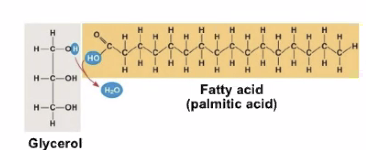
\includegraphics[width=.9\linewidth]{./Screen Shot 2020-09-09 at 2.58.49 PM.png}
\caption{Screen Shot 2020-09-09 at 2.58.49 PM.png}
\end{figure}

A single penteine and embellishments. \textbf{Single Fatty acids = Glycerol}

\subsection{Trygricerol}
\label{sec:org6e72102}
\textbf{Fat! (a.k.a. adapose tissue) = Triglycerol: three fatty acids
together.}

\begin{figure}[htbp]
\centering

\includegraphics[width=.9\linewidth]{Fat_triglyceride_shorthand_formula.png}
\caption{Fat\textsubscript{triglyceride}\textsubscript{shorthand}\textsubscript{formula.png}}
\end{figure}

\subsubsection{Saturated vs. Unsaturated fats}
\label{sec:org83c3c1c}
\textbf{Saturate Fats} \emph{No double bonds} in the carbon chain --- think! butter

\textbf{Unsaturated Fats} \emph{Double bonds} in the carbon chain --- think! olive
oils

Saturated fats has a higher melting point then the unsaturated fats, but
unsaturated fats have double bonds whereas saturated fats have single
bonds only. Why?

\begin{itemize}
\item Double bonds, due to their caused VESPR geometry (and hence the -1
hydrogen), are curved. This makes it harder to stack together, causing
a lower melting point
\item Single bonds, due to their caused VESPR geometry, is flat. This makes
them easier to stack together, causing a higher melting point.
\end{itemize}

\subsection{Phosophilids}
\label{sec:orgeaafb4c}
\textbf{2 fatty acids (hydrophobic) + phosphate group (hydrophillic)}

\begin{figure}[htbp]
\centering
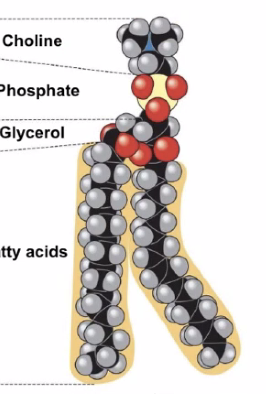
\includegraphics[width=.9\linewidth]{./Screen Shot 2020-09-09 at 3.15.41 PM.png}
\caption{Screen Shot 2020-09-09 at 3.15.41 PM.png}
\end{figure}

A combination of many of these will end up with membrane:
\begin{center}
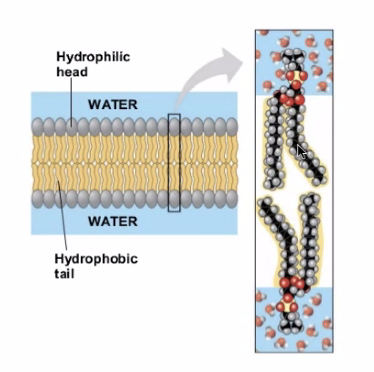
\includegraphics[width=.9\linewidth]{./Screen Shot 2020-09-09 at 3.08.10 PM.png}
\end{center}

The hydrophobic tail stays inside, and the hydrophillic head pokes
outside and attracts water.

\subsection{Liposomes + micelles}
\label{sec:orgc6fd0ef}
\textbf{Lots of phosophillids}

\begin{figure}[htbp]
\centering
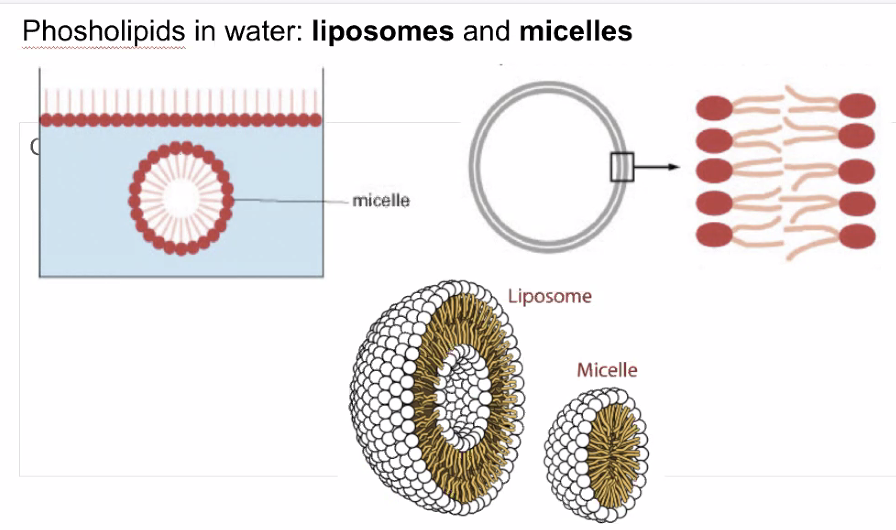
\includegraphics[width=.9\linewidth]{./Screen Shot 2020-09-09 at 3.11.54 PM.png}
\caption{Screen Shot 2020-09-09 at 3.11.54 PM.png}
\end{figure}

A same idea as Phosophilids, but instead in a big wad of Phosolipids.
this arrangement is also how basic cells form membranes.
\href{KBhBIO101CellMembraines.org}{KBhBIO101CellMembraines}

\subsection{Steroids}
\label{sec:orgdafc29b}
\begin{figure}[htbp]
\centering
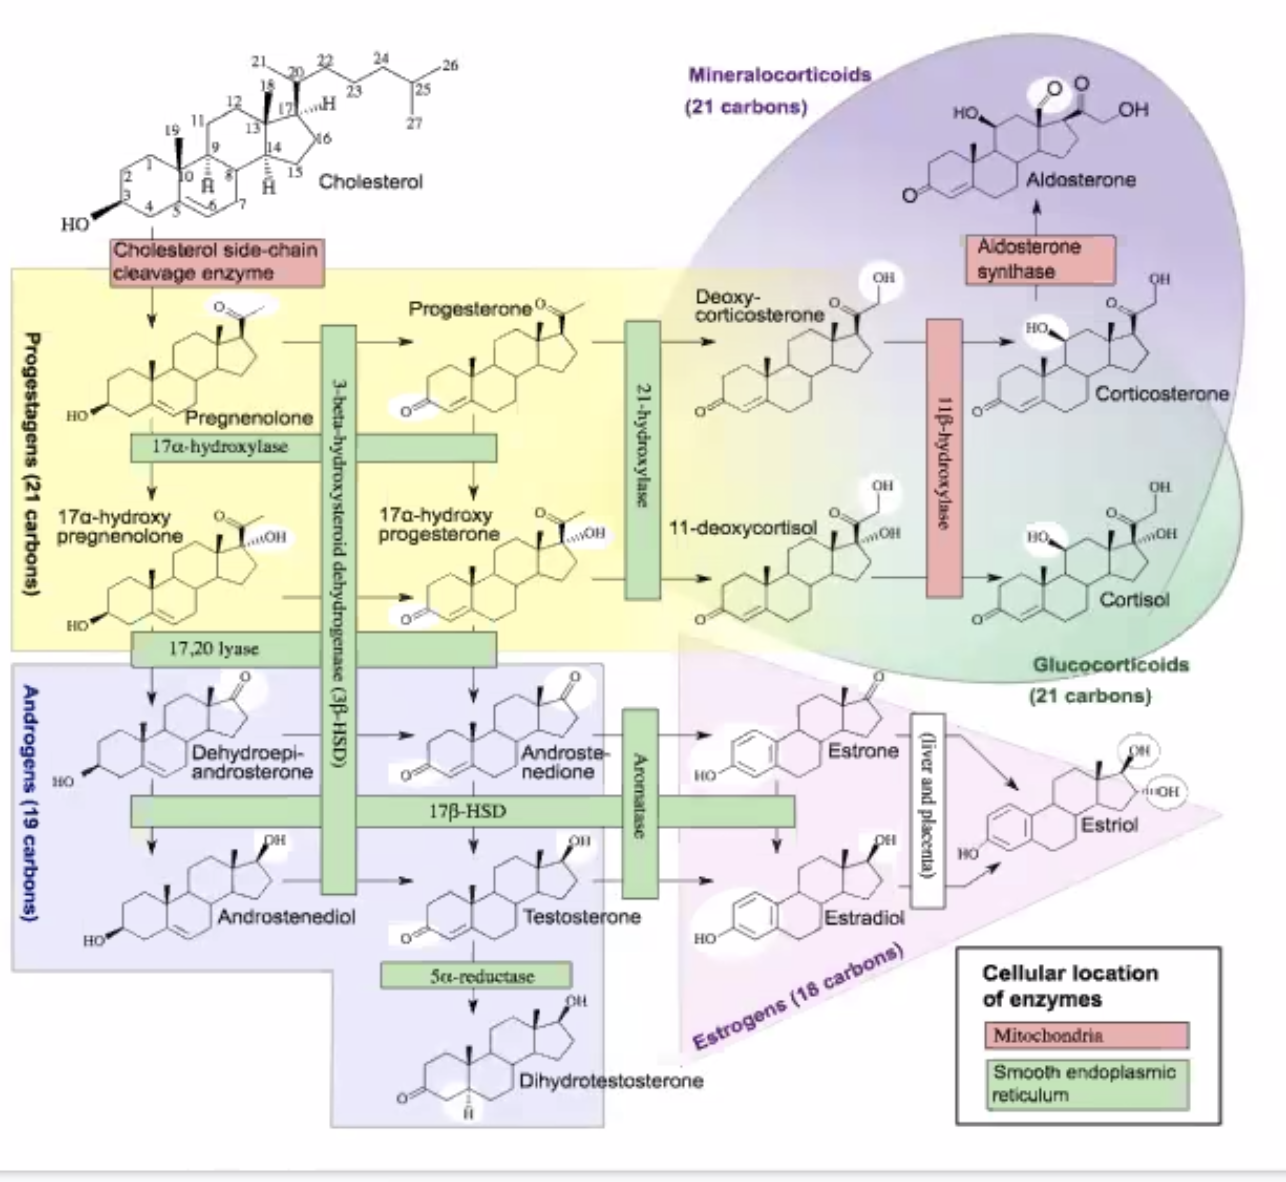
\includegraphics[width=.9\linewidth]{./Screen Shot 2020-09-11 at 2.43.35 PM.png}
\caption{Screen Shot 2020-09-11 at 2.43.35 PM.png}
\end{figure}

Steroids typically are lipids that contain a ring structure, which
usually contains 17 carbon lipids with rings formed by 5-6 carbons each
\end{document}
